%----------------------------------------------------------------------------------------
%       PACKAGES AND OTHER DOCUMENT CONFIGURATIONS
%----------------------------------------------------------------------------------------
\documentclass[paper=letter, fontsize=12pt]{article}
\usepackage[english]{babel} 
\usepackage{amsmath,amsfonts,amsthm} 
\usepackage[utf8]{inputenc}
\usepackage{float}
\usepackage{blindtext}
\usepackage{graphicx} 
\usepackage{caption}
\usepackage{subcaption}
\usepackage[sc]{mathpazo}
\usepackage[T1]{fontenc}
\linespread{1.02}
\usepackage{microtype}
\usepackage[hmarginratio=1:1,left=20mm,top=32mm,columnsep=20pt]{geometry}
\usepackage{multicol}
\usepackage{booktabs}
\usepackage{float}
\usepackage{hyperref}
\usepackage{lettrine}
\usepackage{paralist}
\usepackage{abstract}
\renewcommand{\abstractnamefont}{\normalfont\bfseries}
\renewcommand{\abstracttextfont}{\normalfont\small\itshape}
\usepackage{titlesec}
\usepackage{xcolor}
\usepackage{pgfplots}
\usepackage{listings}
\usepgfplotslibrary{fillbetween}

\titleformat{\section}[block]{\large\scshape\centering}{\thesection.}{1em}{}
\titleformat{\subsection}[block]{\large}{\thesubsection.}{1em}{}
\newcommand{\horrule}[1]{\rule{\linewidth}{#1}}
\usepackage{fancyhdr}
\pagestyle{fancy}
\fancyhead{}
\fancyfoot{}

\definecolor{codegreen}{rgb}{0,0.6,0}
\definecolor{codegray}{rgb}{0.5,0.5,0.5}
\definecolor{codepurple}{rgb}{0.58,0,0.82}
\definecolor{backcolour}{rgb}{0.95,0.95,0.92}

\lstdefinestyle{mystyle}{
    language = Verilog, 
    backgroundcolor=\color{backcolour},   
    commentstyle=\color{codegray},
    keywordstyle=\color{purple},
    numberstyle=\tiny\color{codegray},
    basicstyle=\ttfamily\footnotesize,
    otherkeywords = {logic, 0, 1, 2, 3, 4, 5, 6, 7, 8, 9},
    breakatwhitespace=false,         
    breaklines=false,                 
    captionpos=b,                    
    keepspaces=true,                 
    numbers=left,                    
    numbersep=2pt,                  
    showspaces=false,                
    showstringspaces=false,
    showtabs=false,                  
    tabsize=2
}

\lstset{emph={% 
    call, event
    },emphstyle={\color{blue}\bfseries}
}

\lstset{style=mystyle}

\fancyhead[C]{Politecnico di Milano $\bullet$ Embedded Systems $\bullet$ May 2020 $\bullet$ CSE Track}

\fancyfoot[RO,LE]{\thepage}

\newtheorem{theorem}{Statement}

%----------------------------------------------------------------------------------------
%       TITLE SECTION
%----------------------------------------------------------------------------------------
\title{\vspace{-15mm}\fontsize{24pt}{10pt}\selectfont\textbf{bfloat SQRT module documentation}}
\author{
\large{\textsc{Roberto Rocco, 920721}}\\[2mm]
\large{\textsc{Leonardo Staglianò, 917310}}\\[2mm]
}
\date{}
%----------------------------------------------------------------------------------------

\begin{document}
\maketitle 
\thispagestyle{fancy}

%----------------------------------------------------------------------------------------
%       DOCUMENT SECTION
%----------------------------------------------------------------------------------------

\section{Introduction}
This document explains the structure of the sqrt module for the bfloat fpu. The document is structured as follows: Section~\ref{section:algo} will explain the algorithm and will show some useful properties that have been exploited during the implementation, Section~\ref{section:impl} will analyze in detail the implementation and integration steps, Section~\ref{section:test} will show the result of the tests performed on the module.

\section{Algorithm analysis}
\label{section:algo}
Floating point numbers are represented following the standard IEEE 754 \cite{8766229}. The standard specifies 3 fields (sign, exponent, mantissa) and their value concerning the number that must be represented. The formula \(x = (-1)^S * (1+M) * 2^E\) explains how most numbers are mapped into the standard representation.

Given the above representation, it is possible analyze the impact of the square root operation over the fields: \(\sqrt{x} = \sqrt{(-1)^S} * \sqrt{(1+M)} * \sqrt{2^E} = \sqrt{(-1)^S} * \sqrt{(1+M)} * 2^{E/2}\). From this formulation few observations can be obtained:
\begin{itemize}
    \item If \(S = 1\) there is no solution (it is impossible to obtain square root of a negative number in \(\mathbb{R}\));
    \item If \(S = 0\) it is possible to compute the new values of the fields as follows:
    \begin{equation}
        \label{eq:general}
        \begin{cases}
        S' = S = 0;\\
        M' = \sqrt{(1+M)} - 1;\\
        E' = E/2;\end{cases}
    \end{equation}
    \item Since \(E'\) must be an integer number as \(E\), it's mandatory to consider two separate cases and distinguish whether \(E\) is odd or even. 
    \begin{itemize}
        \item If even, then \(E = 2k\) for some integer k, so \(E' = k\) without further problems;
        \item If odd, then \(E = 2k - 1\) for some integer k. It is then possible to represent the initial number \(x\) as \(x = (1+M) * 2^{2k} * 2^{-1} = \frac{(1+M)}{2} * 2^{2k}\), so its square root value becomes \(\sqrt{x} = \sqrt{\frac{(1+M)}{2}} * \sqrt{2^{2k}} = \sqrt{\frac{(1+M)}{2}} * 2^{k}\).
    \end{itemize}
    \item From all these considerations it is possible to compute the correct values:\\
    \begin{equation}
        \label{eq:specific}
        \begin{cases}
            NaN & \mbox{if }S\mbox{ is 1;}\\[2mm]
            \begin{cases}
                S' = S = 0;\\
                M' = \sqrt{(1+M)} - 1;\\
                E' = E/2;
            \end{cases} & \mbox{if }E\mbox{ is even and }S\mbox{ is 0;}\\
            \begin{cases}
                S' = S = 0;\\
                M' = \sqrt{\frac{(1+M)}{2}} - 1;\\
                E' = \frac{(E - 1)}{2};
            \end{cases} & \mbox{if }E\mbox{ is odd and }S\mbox{ is 0;}
        \end{cases}
    \end{equation}
\end{itemize}

It's easy to see from the above formula that the only non-trivial field is \(M'\). To compute it, it is possible to exploit the Goldschmidt’s algorithm, following the approach proposed in \cite{markstein2004software}. The algorithm consists in these steps:
\begin{itemize}
    \item The initial values are
    \begin{equation}b_0 = v\mbox{; } g_0 = v \label{eq:algo_start}\end{equation}
    where \(v\) represents the value under the square root sign (either \(1+M\) or its half);
    \item At each iteration \(j\), compute \(y_j\) as an estimation of\(\frac{1}{\sqrt{b_{j-1}}}\); then \begin{equation}b_j = b_{j-1} * {y_j}^2\mbox{; } g_j = g_{j-1} * y_j
    \label{eq:algo_iterate}\end{equation}
    \item Repeat until \(b_j\) is equal (or at least close) to 1, \(g_j\) will contain the needed square root. 
\end{itemize}

The effort proposed the use of the tangent to the curve in the point with \(b_j = 1\) as a way to obtain \(y_j\). This way the value of \(y_j\) becomes equal to:
\begin{equation}
    \label{eq:line}
    y_j = \frac{3-b_{j-1}}{2}
\end{equation}

To analyze the precision of the approximation, it's mandatory to define the domain of \(b_j\). In particular, it's possible to demonstrate the following statement:

\begin{theorem}
    \label{domain}
    Using as approximation formula \ref{eq:line}, \(0.5 \le b_j < 2\mbox{ } \forall j\)
\end{theorem}

\begin{proof}
    To demonstrate the statement it is possible to proceed by induction. When \(j = 0\), \(b_j = v\) and \(v\) is either \(1+M\) or its half. \(M\) is a fractional value, so \(0 \le M < 1\). Given this, it's easy to assert that \(0.5 \le v < 2\).
    To demonstrate that \(b_j\) is in the range given that \(b_{j-1}\) is within, it's necessary to analyze their correlation. Following the algorithm, it is possible to compute that \(b_j = b_{j-1} * {\left(\frac{3 - b_{j-1}}{2}\right)}^2\). This function in the interval [0.5; 2) has values smaller than 1 and bigger than 0.5, as can be seen in figure \ref{figure:fixed}.
\end{proof}

\begin{figure}
\centering
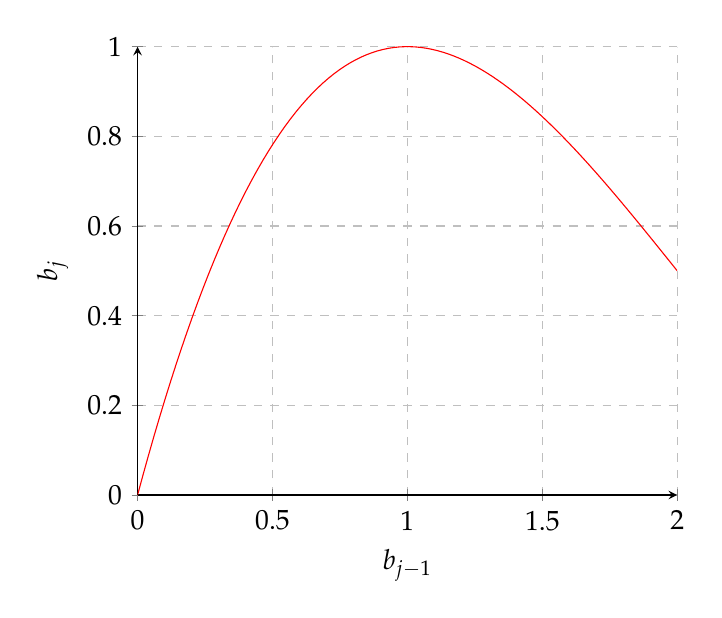
\begin{tikzpicture}
\begin{axis}[
    axis lines = left,
    xlabel = $b_{j-1}$,
    ylabel = ${b_j}$,
    xmajorgrids=true,
    ymajorgrids=true,
    grid style=dashed,
]
\addplot [
    domain=0:2, 
    samples=100, 
    color=red,
]
{x*(x-3)^2/4};
\end{axis}
\end{tikzpicture}
\caption{Study on the function \(b_j\).}
\label{figure:fixed}
\end{figure}

\begin{figure}
    \centering
    \begin{minipage}{0.45\textwidth}
        \centering
        \begin{tikzpicture}
            \begin{axis}[
                axis lines = left,
                xlabel = $x$,
                ylabel = ${f(x)}$,
                xmajorgrids=true,
                ymajorgrids=true,
                grid style=dashed,
                ymax=6
                ]
                \addplot [
                    name path=A,
                    domain=0.0000001:2, 
                    samples=256, 
                    color=red,
                ]
                {x^(-0.5)};
                \addplot [
                    name path=B,
                    domain=0:2, 
                    samples=256, 
                    color=blue,
                ]
                {(3-x)/2};
                \addplot[fill opacity=0.2] fill between[of=A and B,];
            \end{axis}
        \end{tikzpicture}
        \caption{Comparison between first approximation and real value.}
        \label{figure:approx}
    \end{minipage}\hfill
    \begin{minipage}{0.45\textwidth}
        \centering
        \begin{tikzpicture}
            \begin{axis}[
                axis lines = left,
                xlabel = $x$,
                ylabel = ${f(x)}$,
                xmajorgrids=true,
                ymajorgrids=true,
                grid style=dashed,
                ymax=6
                ]
                \addplot [
                    name path=A1,
                    domain=0.0000001:0.11111, 
                    samples=256, 
                    color=red,
                ]
                {x^(-0.5)};
                \addplot [
                    name path=A2,
                    domain=0.11111:0.36325, 
                    samples=256, 
                    color=red,
                ]
                {x^(-0.5)};
                \addplot [
                    name path=A3,
                    domain=0.36325:2, 
                    samples=256, 
                    color=red,
                ]
                {x^(-0.5)};
                \addplot [
                    name path=B,
                    domain=0.36325:2, 
                    samples=256, 
                    color=blue,
                ]
                {(3-x)/2};
                \addplot[
                    domain=0:0.36325, 
                    samples=256, 
                    color=blue,
                    dashed
                ]{(3-x)/2};
                \addplot[
                    name path=C,
                    domain=0.11111:0.36325, 
                    samples=256, 
                    color=blue,
                ]{2};
                \addplot[
                    name path=D,
                    domain=0.0000001:0.11111,
                    samples=256, 
                    color=blue,
                ]{4};
                \addplot[fill opacity=0.2] fill between[of=A3 and B,];
                \addplot[fill opacity=0.2] fill between[of=A2 and C,];
                \addplot[fill opacity=0.2] fill between[of=A1 and D,];
            \end{axis}
        \end{tikzpicture}
        \caption{Comparison between second approximation and real value.}
        \label{figure:approx2}
    \end{minipage}
\end{figure}

Once the domain is obtained, it's possible to evaluate the approximation by comparing it with the correct value. Figure \ref{figure:approx} plots the two values in the domain. As can be seen in the graph, the approximation is good since the distance between the two curves in the domain is small.

\subsection{Special cases}

The IEEE 754 standard specifies also the representation of values that cannot be obtained in the previous way. It includes infinites, zeros, \(NaN\) and denormalized numbers. The first three can be threated without relevant problems (only positive values are considered, since negative ones will become \(NaN\)):
\begin{itemize}
    \item \(\sqrt{0} = 0\);
    \item \(\sqrt{\infty} = \infty\);
    \item \(\sqrt{NaN} = NaN\).
\end{itemize}
The case of denormalized numbers is trickier: those numbers are mapped following the formula \(x = (-1)^S * M * 2^{-126}\). From that, it's easy to come up to a formulation similar to the one of Formula \ref{eq:specific}:

\begin{equation}
    \label{eq:1.3}
    \begin{cases}
        NaN & \mbox{if }S\mbox{ is 1;}\\[2mm]
        \begin{cases}
            S' = S = 0;\\
            M' = \sqrt{M};\\
            E' = E/2 = -63;
        \end{cases} & \mbox{if }S\mbox{ is 0;}\\
    \end{cases}
\end{equation}

It shall be noted, however, that the result of the operation produces a number that is no more denormalized: some additional operations may be needed to make it coherent with the normal representation. The procedure for the calculation of the square root is similar except for the starting domain: rather than going from 0.5 to 2 excluded, it goes from 0 excluded to 1 excluded. Statement \ref{domain} can be adapted to include those points, since the demonstration would be the same. It becomes:

\begin{theorem}
    \label{domain2}
    Using as approximation formula \ref{eq:line}, \(0 < b_j < 2\mbox{ } \forall j\)
\end{theorem}

The new domain introduces problems with the current approximation chosen: in the interval (0; 0.5) the error is relevant. A bad approximation would lead to the result after more iterations, so it would slow down the component. A better approximation is needed, at least for some part of the domain. A good approximation function must present a low error and must be simple to compute: complex operations shall be avoided since they may require a lot of time to complete and would slow down the component.

Given all the above requirements, and given that the function \ref{eq:line} solves the problem in the domain [0.5;2), it's natural to use it together with some others that would handle the problematic part. The solution adopted uses the following function:

\begin{equation}
    \label{eq:comp_line}
    y_i = \begin{cases}
        4 & \mbox{if }b_{j-1} \le \frac{1}{9}\\
        2 & \mbox{if } \frac{1}{9} < b_{j-1} < 0.36325\\
        \frac{3-b_{j-1}}{2} & \mbox{if } b_{j-1} \ge 0.36325
    \end{cases}
\end{equation}

It shall be remarked that the values \(\frac{1}{9}\) and \(0.36325\) are chosen to reduce to the minimum the distance between the function and its approximation. Domain analysis must be done again since the approximation function is different.

\begin{theorem}
    \label{domain3}
    Using as approximation formula \ref{eq:comp_line}, \(0 < b_j < 2\mbox{ } \forall j\)
\end{theorem}

\begin{proof}
    It's still possible to proceed by induction. The base case is the same as Statement \ref{domain2}. Proving that \(b_j\) is within the range if \(b_{j-1}\) is part of it can be done splitting the three cases:
    \begin{itemize}
        \item if \(b_{j-1} \ge 0.36325\), the situation is analogous to Statement \ref{domain2};
        \item if \(\frac{1}{9} < b_{j-1} < 0.36325\), then \(b_j = 4b_{j-1}\). Since \(b_{j-1} > 0\), \(b_j > b_{j-1} > 0\). The maximum value \(b_j\) can reach is \(4 * 0.36325 = 1.453 < 2\);
        \item in a similar way, if \(\frac{1}{9} \ge b_{j-1}\), then \(b_j = 16b_{j-1}\). The maximum value \(b_j\) can reach is \(16 * \frac{1}{9} = 1.\overline{7} < 2\).
    \end{itemize}
\end{proof}

It's possible to plot this new approximation function and compare it with the other. This has been done in Figure \ref{figure:approx2}, where it can be seen that the grey area (corresponding to the error) is smaller compared with the one in Figure \ref{figure:approx}. Moreover, the constant values are very fast to use and the impact on the component is small.

\subsection{Inverse calculation}

The algorithm proposed in \cite{markstein2004software} allows also the calculation of the inverse of the result. To obtain such a result, the algorithm must be slightly changed to introduce another variable. The new variable is called \(i_j\)\footnote{It shall be noted that in \cite{markstein2004software} it is named \(y_j\) and the variable that here has its name is called \(Y_j\). It has been decided to change the name to avoid confusion between the two.}: 
\begin{equation}
\begin{cases}
i_0 = 1\\
i_j = i_{j-1} * y_j
\end{cases}
\label{eq:inverse}
\end{equation}
The needed value will be contained in \(i_j\) when the algorithm ends. This calculation doesn't change the previous considerations on the approximations.

\section{Implementation}
\label{section:impl}
In the following section, all the implementation details of the above algorithms will be analyzed, including how it was possible to introduce some mathematical approximations that have a meaningful performance impact. The first part will provide some details on the bfloat representation and will be followed by a punctual exposition of the implementation of the algorithm and some additional notions on truncation and integration.
\subsection{Data representation}
The operand of the module is stored and elaborated through the \texttt{bfloat16} representation which is based on the IEEE 754 standard on 32 bits as described in \cite{8766229}. The modification concerning the usual representation on 32 bits regards mainly the number of bits in which each field is codified, \texttt{bfloat16} numbers are represented as follows:
\begin{itemize}
    \item S (sign): 1 bit
    \item E (exponent): 8 bits
    \item M (mantissa): 7 bits
\end{itemize}

Since the number of bits for the exponent is the same as in the original IEEE 754 specification over 32 bits, all the considerations about the bias of such field of the number remain valid.\newline
One important detail about this representation is that the 7 bits of the mantissa represent only the fractional part of the number: to obtain the real mantissa, the value shall be preceded by either an integer 1 or 0, depending on the normalization of the number. 
The module operates on the entire number so the fields that are provided in the input have the very same dimensions of the representation above, except for the mantissa which has 8 bits to include the implicit integer digit.

Firstly it is useful to analyze the module interface:
\begin{lstlisting}
input                                       clk,
input                                       rst, 
input logic                                 doSqrt_i,
input logic [(7+1)-1:0]                     extF_op1_i,
input logic [8-1:0]                         e_op1_i,
input logic                                 s_op1_i,
input logic                                 isZ_op1_i,
input logic                                 isInf_op1_i,
input logic                                 isSNaN_op1_i,
input logic                                 isQNaN_op1_i,
input logic                                 isOpInv_i,

output logic                                s_res_o,
output logic [8-1:0]                        e_res_o,
output logic [(7+2+3)-1:0]                  f_res_o,	
output logic                                valid_o,
output logic                                isToRound_o
\end{lstlisting}
A brief explanation of the functionality of each input is provided in the following list:
\begin{itemize}
    \item \texttt{clk}: the clock signal;
    \item \texttt{rst}: the reset signal;
    \item \texttt{doSqrt\_i}: the signal that indicate whether the inputs are stable and the calculation can start;
    \item \texttt{extF\_op1\_i}: the signal which contains the implicit bit and the mantissa of the operand;
    \item \texttt{e\_op1\_i}: the signal which contains the exponent of the operand;
    \item \texttt{s\_op1\_i}: the signal which contains the sign of the operand;
    \item \texttt{isZ\_op1\_i}, \texttt{isInf\_op1\_i}, \texttt{isNaN\_op1\_i}, \texttt{isQNaN\_op1\_i}: signaling bits to handle exceptional cases;
    \item \texttt{isOpInv\_i}: signaling bit to toggle the calculation of the inverse square root;
\end{itemize}
The following list does the same for the output:
\begin{itemize}
    \item \texttt{s\_res\_o}: the output sign
    \item \texttt{e\_res\_o}: the output exponent
    \item \texttt{f\_res\_o}: the output fractional number, which includes: the mantissa (7 bits), the implicit integer digit (1 bit) and the bits for rounding (3 bits)
    \item \texttt{valid\_o}: a signaling bit for stable output availability
    \item \texttt{isToRound\_o}: a signaling bit that is low only in the exceptional cases (Zero, Inf, NaN)
\end{itemize}
During the computation, the operands that contribute at the calculation of the resulting (extended) mantissa may need additional bits to perform a correct rounding in the top module. The following line of code shows an example of SystemVerilog logic declaration:
\begin{lstlisting}
logic [(7+1+3)-1:0]           b_r, b_next;
\end{lstlisting}
As can be seen above, the b register has 7 bits (the same number of bits that composes the mantissa of the input), plus 1 for the integer digit and other three bits (guard, sticky and round bits) for rounding purposes. All the other registers dimensions can be explained in an analogous way, with the exception of some that may contain results of multiplications: in those cases, the dimension may be multiplied by a factor correlated to the number of operands involved. The exception is showed in the below example:
\begin{lstlisting}
logic [2*(7+1+3)-1:0]         y_square_r, y_square_next;
\end{lstlisting}
The \texttt{y\_square\_r} register contains the result of the multiplication of 2 numbers that are contained into register of the same dimension of \texttt{b\_r}, so it's size will be double with respect to \texttt{b\_r}.
\subsection{Algorithm realization}
To better understand the implementation, it is useful to first explain the meaning of the registers and wires later mentioned. Those refer to the mathematical counterparts that are present in \cite{markstein2004software} and explored in Section \ref{section:algo}. To save partial results across the iterations, the storing feature of the Verilog registers is exploited.
\begin{itemize}
    \item \texttt{ss\_r}: the state register;
    \item \texttt{b\_r, y\_r,  g\_r}: they correspond to the b, y, g operands;
    \item \texttt{i\_r}: used to store the partial mantissa of the inverse square root of the input operand;
    \item \texttt{s\_r}: stores the sign of the result (immediately calculated);
    \item \texttt{e\_r}: stores the exponent of the result (immediately calculated);
    \item \texttt{iteration\_r}: stores the number of times the Goldschmidt algorithm is applied;
    \item \texttt{i\_ib\_r}: it is used to handle the possible increment (across multiple iterations) of digits needed to store the integer part of the inverse;
    \item \texttt{isSNaN\_r, isQNaN\_r, isZ\_r, isInf\_r, isInv\_r}: used to store the homonyms input signal to achieve stability of the input interface of the module;
    \item \texttt{g\_temp\_r}: a wire that is used for the partial computation of the g number. It allows to perform a correct truncation across iterations, handling the extra bits of the product of the previous value of g and y inside its larger dimension;
    \item \texttt{i\_temp\_r}: a wire used for the mantissa computation of the inverse result, to be able to perform truncation as above;
    \item \texttt{y\_temp\_r}: a wire to perform the truncation of the y at each iteration as expressed in \ref{eq:line};
    \item \texttt{y\_square\_r}: as the name says, it is used to be able to to calculate the next value to be stored in the register b, whom calculation requires y squared \ref{eq:algo_iterate};
    \item \texttt{lzeros\_r, lzeros\_inv\_r}: used to perform correct shifting of the results before the output phase and consequently involved in the adjustment of the exponent of the result;
    \item \texttt{e\_div2\_r}: used to handle the adjustment of the bias of the exponent once halved by the shifting detailed below;
\end{itemize} 

The algorithm has been realized using a state machine. It features four states: \texttt{IDLE}, \texttt{WORK}, \texttt{CALC}, \texttt{RESULT}. The first one will wait for the proper signal to start preparing all the registers for the computation and move to the next state, following the analysis of the inputs as in the equation \ref{eq:specific}. The sign of the operand is checked to pull up the NaN signal in case it would be negative, and if the condition doesn't hold all the other "side-cases" (Zero, NaN, Inf codifications) are checked to skip the real computation and jump directly to the state in which the result is ready. In case no exceptional cases are encountered the following steps are performed:
\begin{itemize}
    \item The extended mantissa of the operand is stored into the b register that will also include 3 additional bits to perform truncation (later discussed in this document). It is important to notice that the operand is properly shifted to handle the case in which an odd exponent is given in input since it would lead to a fractional exponent in the result as it has to be halved.
\begin{lstlisting}
b_next = (e_op1_i[0] || (e_op1_i == '0)) ? {extF_op1_i, 3'd0} : {1'd0, extF_op1_i, 2'd0};
\end{lstlisting}
    As can be seen from the code above, the shift operation is not described explicitly by the usage of the Verilog operator \texttt{>>}, instead the constructor operator is used to arrange the bits in the way they have to be stored into the register to correctly represent the desired number.
    \item The partial exponent is calculated by shifting the original of one position to the right, the odd case is already considered because the possible implicit truncation is handled as explained above.
    \item The bias of the exponent is restored (since it was halved too) by adding the half of the bias to the partial result previously obtained. The final exponent is thus stored into the register.
\begin{lstlisting}
e_r_next = ~(isOpInv_i) ? e_div2_r + 64 : 190 - e_div2_r;
\end{lstlisting}
    As shown above, in the "normal" square root operation the bias of the exponent is restored by adding its half plus one. In the inverse case, it is necessary not only to obtain the number with the correct bias but also its opposite.
    \item The \texttt{i\_r} register is initialized with the string \texttt{10000000000}, which codifies 1.0 in the extended representation of the implicit 1 and the fractional part extended with the three extra bits used for truncation.
    \item As a consequence of what is said above, the i\_ib register has to be set to 1 since the number of integers to represent the integer part of the mantissa of the result is exactly one.
    \item The register that keeps track of the number of iterations is initialized to 0.
\end{itemize}

In the next state, \textbf\texttt{WORK}, many operations useful for the following state execution are performed. Sometimes, the execution will be handled completely in this state for an iteration: this happens when y is equal to 2 or 4 following the formula \ref{eq:comp_line}. This special case will be analyzed first, and will be followed by the normal flow which leads to the \texttt{CALC} state.
\begin{itemize}
    \item The first thing checked is if \texttt{y\_r} is approximated as a constant or the tangent. In the first case the y register is replaced by one of the two constants: those are chosen to gain advantages in terms of computational complexity of the operations (divisions mostly), since having constants (2 and 4 in the specific case) that are power of 2 leads to the possibility of doing a shift operation instead of a multiplication or a division. This case is handled by shifting the b and g register by an appropriate number of positions that depends on the constants. The inverse case is considered by simply adding the shifting constant to the \texttt{i\_bi\_r} register.
\begin{lstlisting}
//Y is clamped to 4
b_next = b_r << SHIFT_CONST4*2;
g_next = g_r << SHIFT_CONST4;
i_ib_next = i_ib_r + SHIFT_CONST4;
\end{lstlisting}
    \item The second case performs only the calculation of the new value of y and y square applying the formula \ref{eq:line}.
\begin{lstlisting}
y_temp_r = 12'b110000000000 - ({1'b0, b_r});
y_next = {y_temp_r[11:2], y_temp_r[1]};
y_square_next = {y_temp_r[11:2], y_temp_r[1]} * {y_temp_r[11:2], y_temp_r[1]};
ss_next = CALC;
\end{lstlisting}
    \end{itemize}
    
The state \textbf\texttt{CALC} is responsible for the finalization of all the computations needed to compute an iteration. It's reached only if the \texttt{WORK} state used the tangent.
    \begin{itemize}
    \item The \texttt{y\_square\_r} register is used in combination with the current value of b to compute the value of b for the next iteration. Slicing is required, since the multiplication of those three values has three integer digits as result, but the representation requires only a single integer bit.
\begin{lstlisting}
b_partial_r = b_r * y_square_r;
b_next = b_partial_r[30 -: 11];
\end{lstlisting}
    The new value of the \textbf\texttt{b\_r} register is obtained taking 11 bits (its dimension) starting from the bit 31: this means that, since the \textbf\texttt{b\_partial\_r} register is 33 bits long, the first two bits (that represents 2 of the 3 integer digit) are discarded. 
    \item The register that contains g is updated following the formula \ref{eq:algo_iterate}. Here the truncation to the intermediate result of the multiplication is applied.
    \item The remaining operations are all about the inverse calculation: the partial product of \texttt{y\_r} register times the \texttt{i\_r} register is computed and processed to eliminate possible zeros in the most significant bits; the \texttt{i\_ib\_r} register is updated accordingly; the final result is, as usual, obtained after a truncation.
\begin{lstlisting}
i_temp_r = (i_r * y_r);
lzeros_inv_r = FUNC_numLeadingZeros(i_temp_r[21-:8]);
i_ib_next = i_ib_r + 1 - lzeros_inv_r;
i_temp_r = i_temp_r << lzeros_inv_r;
i_next = {i_temp_r[21 -:10], |i_temp_r[10-:STICKYANALYSIS]};
\end{lstlisting}
    \end{itemize}
The next state will be selected according to few conditions. If the register \texttt{b\_r} contains \texttt{10000000000} or the maximum number of iterations is reached, then the module is ready to produce its result (or has no more time to get a better one): execution will continue to the \texttt{RESULT} state. If those conditions don't apply, then computation must proceed and the next state will be \texttt{CALC} again.

The last state of the implementation is \textbf{RESULT}, which is responsible for the management of the output.
\begin{itemize}
    \item The corner cases are checked and the result is prepared to be compliant with the BFLOAT representation. (Zero, Inf, NaN);
    \item In case the required operation is the inverse of the square root, it is not necessary to perform any post processing on the i register, since the possible presence of leading zeros is already handled in the previous states, so it represents the final mantissa of the result. The \texttt{i\_ib\_r} register is used to compute the correct exponent by adding to it the content of the \texttt{i\_ib\_r} register.
\begin{lstlisting}
s_res_o = s_r;
e_res_o = e_r + i_ib_r - 1;
f_res_o = {1'b0, i_r};
\end{lstlisting}
    \item The normal square root result is prepared through a post processing that counts the number of leading zeros, shifts the mantissa properly and updates the exponent accordingly.
\begin{lstlisting}
lzeros_r = FUNC_numLeadingZeros(g_r[10-:8]);
s_res_o = s_r;
e_res_o = e_r - lzeros_r;
f_res_o = {1'b0, g_r << lzeros_r};
\end{lstlisting}
\end{itemize}
The additional zero added as most significant bit in the mantissa of the result is due to the need of being compliant with the representation of the top module, as it signals a possible overflow, never present in our cases. 

Execution then continues into the \texttt{IDLE} state.

\subsection{Rounding and truncation}
Some operations executed by our module make the result bigger than the register that will hold the value: multiplications tend to expose this behavior. To make the result fit, the truncation must be performed, but it introduces rounding error. To reduce its impact, guard, round and sticky bits have been introduced. Moreover, to allow better optimization, it is possible to configure the module to change the span over which the sticky bit is computed: the \texttt{STICKYANALYSIS} constant is used for this. A simple example of this concept can be seen in the code snippet below:
\begin{lstlisting}
g_temp_r = (g_r * y_r);		 
g_next = {g_temp_r[20 -:10], |g_temp_r[10-:STICKYANALYSIS]};
\end{lstlisting}

\texttt{g\_r} is updated storing a truncated and rounded version of the product that has as operands \texttt{g\_r} itself and \texttt{y\_r}. The intermediate result has 22 bits (each operand has 11 bits) in which 2 bits represent the integer part of the obtained number and the other 20 bits give its fractional part. To store a value in \texttt{g\_r} we have to go back to a representation on 11 bits so we take just one integer bit (the less significant since the most one will always be 0) and the fractional bits are taken in this way: the first 10 are taken exactly from the intermediate result, the last bit is obtained by applying a bitwise-or to the next \texttt{STICKYANALYIS} bits starting from the number 10. This implies that the "extra" fractional part that results from the product is approximated considering only some of the most significant bits, the others are simply discarded.

The rounding operations on the final result will be completed in a more general module.

\subsection{Integration with the current FPU}
The integration of the module with the other components that make up the entire FPU can be summarized by inspecting the following Verilog instantiation taken from the top module:
\begin{lstlisting}
lampFPU_sqrt
        lampFPU_sqrt0 (
            .clk                    (clk),
            .rst                    (rst),
            //  inputs
            .doSqrt_i               (doSqrt_r),
            .extF_op1_i             (extF_op1_r),
            .e_op1_i                (e_op1_r),
            .s_op1_i                (s_op1_r),
            .isZ_op1_i				(isZ_op1_r),
            .isInf_op1_i            (isInf_op1_r),
            .isSNaN_op1_i           (isSNAN_op1_r),
            .isQNaN_op1_i           (isQNAN_op1_r),
            .isOpInv_i              (isOpInv_r),
            //  outputs
            .s_res_o                (sqrt_s_res),
            .e_res_o                (sqrt_e_res),
            .f_res_o                (sqrt_f_res),
            .valid_o                (sqrt_valid),
            .isToRound_o            (sqrt_isToRound)
        );
\end{lstlisting}
\begin{itemize}
    \item The clk and the rst signal are connected to the clock and reset port of the sqrt module.
    \item The input signal that triggers the functioning of the FP unit is connected to the port that starts the computation of the sqrt module.
    \item The \texttt{extF\_op1\_i} port is connected to the \texttt{extF\_op1\_r} register that we can find in the pre-processing part of the top module as the one that contains the extended mantissa of the original operand, the extension simply adds the implicit integer digit to the fractional part of the number (0 is denormalized, 1 otherwise). 
    \item An analogous reasoning can be done for \texttt{e\_op1\_r}, \texttt{s\_op1\_r}, \texttt{isZ\_op1\_i}, \texttt{isInf\_op1\_i}, \texttt{isSNaN\_op1\_i} and \texttt{isQNaN\_op1\_i} as they connect the registers that contain the sign and the exponent of the operand to the corresponding ports of the module. All the registers involved are, once again, taken from the pre-processing part of the top module which analyzes the operand in input with respect to the standard representation.
    \item \texttt{isOpInv\_r} is connected to the port of the module which states whether either the square root or the inverse square root is required.
    This register is set to 1 in case the Opcode given in input to the FU specifies the inverse square root operation.
    \item The output ports \texttt{s\_res\_o}, \texttt{e\_res\_o}, \texttt{f\_res\_o} are connected to the wires used in the post-processing part of the top module, this means that they bring the outputs to the rounding logic that prepares the data before the final result is given in output.
    \item \texttt{valid\_o} port is connected to the wire that will drive the top module to effectively output the final value.
    \item \texttt{isToRound\_o} port is connected to the signal that triggers the rounding process in case of necessity.
\end{itemize}
As it can be seen from the above explanation the integration of the module has required the introduction of the following wires:
\begin{lstlisting}
logic                                   sqrt_s_res;
logic [(LAMP_FLOAT_E_DW)-1:0]           sqrt_e_res;
logic [(LAMP_FLOAT_F_DW+2+3)-1:0]       sqrt_f_res;
logic                                   sqrt_valid;
logic                                   sqrt_isToRound;
\end{lstlisting}
Their purpose is to correctly bring the result of the sqrt module to the other logics present in the top implementation.

\section{Testing and evaluation}
\label{section:test}

The module was integrated into the tests of the other modules. This allows to check the functioning of the module and evaluate its precision. The testing is analogous to the other modules: it generates a random floating-point number and computes its square root both with the implemented module and the fpu of the simulator (via a c file). It then compares the two results, pointing out an error if they are different. Specific analysis for the denormalized number is also performed to better analyze their impact on the correctness of the module.

Testing is exploited to optimize the value of certain design parameters. The optimization is toward the error percentage reduction: the total absence of errors cannot be achieved, since the simulator operates with 32-bit floats, while the module only uses 16-bit. The optimization must also consider the variables that can affect the precision: rounding policy is one of these.

To prove the validity of the implemented module, its error percentage must be comparable with the one of other similar operations, such as multiplication and division.

The module configurations analyzed are:
\begin{itemize}
    \item Configuration 1: all the exceeding bits are used for the computation of the sticky bit, approximation using formula \ref{eq:line};
    \item Configuration 2: all the exceeding bits are used for the computation of the sticky bit, approximation using formula \ref{eq:comp_line};
    \item Configuration 3: only one exceeding bit is used for the computation (like truncation), approximation using formula \ref{eq:line};
    \item Configuration 4: only one exceeding bit is used for the computation (like truncation), approximation using formula \ref{eq:comp_line};
    \item Configuration 5: first three exceeding bits are used for the computation of the sticky bit, approximation using formula \ref{eq:comp_line};
    \item Configuration 6: first six exceeding bits are used for the computation of the sticky bit, approximation using formula \ref{eq:comp_line};
\end{itemize}
Each configuration will be tested four times, analyzing both normal and denormalized numbers with both the rounding policies supported (truncation and round to nearest). Results of those tests can be seen in Figure \ref{figure:sqrt_bar} and \ref{figure:isqrt_bar}.

From those figures, it's easy to see that the configurations are not all valid: the first and the second, in particular, have a too high error percentage on all the tests done on the ISQRT operation. Among the others, the fourth configuration is better than the third. The last three configurations have different results: the test on the ISQRT operation prefer the fourth configuration, the ones on SQRT depend on the rounding policy. Since neither the operation nor the rounding policy is fixed a-priori, the adopted configuration shall perform reasonably well on any situation: that's the reason why configuration 4 has been chosen for the module.

Timing analysis is crucial since it must be assured that the module can behave correctly given a certain clock frequency. The post-synthesis timing analysis of the overall FPU containing the SQRT module met all the timing constraints (10ns period clock), reporting a worst negative slack (WNS) of 0.15ns. 

\pgfplotstableread[row sep=\\,col sep=&]{
    configuration & TN   & TD   & RN   & RD   \\
    %mult          &  0.0 &  0.0 & 38.0 &  0.0 \\    
    %div           &  7.0 &  0.0 & 27.0 &  0.0 \\    
    C1            & 42.0 & 35.0 & 60.0 & 66.0 \\    
    C2            & 42.0 & 17.0 & 60.0 & 54.0 \\    
    C3            & 10.0 & 47.0 & 25.0 & 49.0 \\    
    C4            & 10.0 & 28.0 & 25.0 & 37.0 \\    
    C5            &  9.0 & 25.0 & 37.0 & 53.0 \\    
    C6            & 14.0 & 22.0 & 43.0 & 59.0 \\
    }\mydata
\begin{figure}
    \begin{tikzpicture}
        \begin{axis}[
                ybar,
                bar width=.5cm,
                width=\textwidth,
                height=.5\textwidth,
                symbolic x coords={C1,C2,C3,C4,C5,C6},
                xtick=data,
                nodes near coords,
                nodes near coords align={vertical},
                ymin=0,ymax=100,
                ylabel={$error\%$},
            ]
            \addplot table[x=configuration,y=TN]{\mydata};
            \addplot table[x=configuration,y=TD]{\mydata};
            \addplot table[x=configuration,y=RN]{\mydata};
            \addplot table[x=configuration,y=RD]{\mydata};
            \legend{Trunc norm, Trunc denorm, Round norm, Round denorm}
        \end{axis}
    \end{tikzpicture}
    \caption{Comparison of the various configurations with SQRT operation.}
    \label{figure:sqrt_bar}
\end{figure}
\pgfplotstableread[row sep=\\,col sep=&]{
    configuration & TN   & TD   & RN   & RD   \\
    %mult          &  0.0 &  0.0 & 38.0 &  0.0 \\    
    %div           &  7.0 &  0.0 & 27.0 &  0.0 \\    
    C1            & 62.0 & 67.0 & 93.0 & 66.0 \\    
    C2            & 62.0 & 59.0 & 93.0 & 74.0 \\    
    C3            & 11.0 & 21.0 & 40.0 & 46.0 \\    
    C4            & 11.0 &  9.0 & 40.0 & 41.0 \\    
    C5            & 16.0 & 32.0 & 49.0 & 45.0 \\    
    C6            & 25.0 & 35.0 & 53.0 & 47.0 \\
    }\mydatum
\begin{figure}
    \begin{tikzpicture}
        \begin{axis}[
                ybar,
                bar width=.5cm,
                width=\textwidth,
                height=.5\textwidth,
                symbolic x coords={C1,C2,C3,C4,C5,C6},
                xtick=data,
                nodes near coords,
                nodes near coords align={vertical},
                ymin=0,ymax=100,
                ylabel={$error\%$},
            ]
            \addplot table[x=configuration,y=TN]{\mydatum};
            \addplot table[x=configuration,y=TD]{\mydatum};
            \addplot table[x=configuration,y=RN]{\mydatum};
            \addplot table[x=configuration,y=RD]{\mydatum};
            \legend{Trunc norm, Trunc denorm, Round norm, Round denorm}
        \end{axis}
    \end{tikzpicture}
    \caption{Comparison of the various configurations with ISQRT operation.}
    \label{figure:isqrt_bar}
\end{figure}

%----------------------------------------------------------------------------------------
%       BIBLIOGRAPHY
%----------------------------------------------------------------------------------------

\bibliographystyle{acm}
\bibliography{references}

%----------------------------------------------------------------------------------------


\end{document}
